\chapter{Object dynamics}\label{chap:object_dynamics}

	Contents of this chapter include an overview of physical laws and astronomical systems and algorithms describing movement of space debris objects which have the biggest impact on further contents of this thesis.

\section{Kepler's laws of orbital motion}\label{sec:kepler}
	
	Kepler's law of orbital motion describes motion of a satellite in regards to gravitational centre of mass, e.g. Sun to the centre of the galaxy, Earth to Sun, etc. Generally, it states that such motion follows a trajectory which is always elliptically shaped.
	
	In astronomy, an object's position in an inertial system, e.g. geocentric or heliocentric, at specific time (reference epoch $t$) can be defined from two different angles.
	
	Either we define a state vector (three position vector components and three velocity vector components) or we define six orbital elements for an elliptical type of orbit:
	
	\begin{itemize}
		\item $a$ - semi-major axis [m]
		\item $e$ - eccentricity [-]
		\item $i$ - orbital inclination [°]
		\item $\Omega$ - right ascension of ascending node (RAAN) [°]
		\item $\omega$ - argument of pericenter/perigee
		\item $M_t$ - mean anomaly at reference epoch $t$ [°]
	\end{itemize}
	
	Elements $a$ and $e$ define shape of the ellipse while $i$ and $\Omega$ define orientation of the elliptical plane, $\omega$ defines the orientation of the ellipse in the elliptical plane and $M_t$ defines position of an object on the ellipse \citep{montenbruck2005satellite}.

\section{Equatorial coordinate system}\label{sec:ra_dec}
	
	To describe an object's position on celestial sphere, we use astronomical coordinate system called Equatorial coordinates defined through two parameters, right ascension (RA, $\langle\ang{0},\ang{360}\rangle$) and Declination (Dec, $\langle\ang{-90},\ang{90}\rangle$). This coordinate reference system is fixed on Earth's equator and vernal equinox \citep{montenbruck2005satellite}. See Figure \ref{fig:equatorial} for an illustration of RA/Dec with regards to Earth.
	
	\begin{figure}[H]
	\centering
	  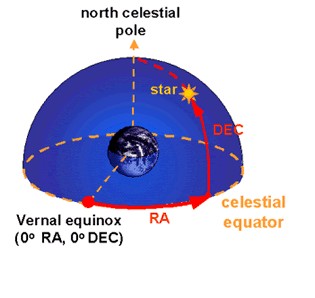
\includegraphics[width=6cm]{images/equatorial}
		  \caption{RA/Dec illustrated.}
	  \label{fig:equatorial}
	\end{figure}

\section{CCD and image reference frame}\label{sec:ccd}

	The first product of an observation is an object's position in the CCD reference frame ($x$, $y$). To transform from the $x$ and $y$ coordinates to RA/Dec a so called \emph{astrometric reduction} is employed which, in general, means linking the two systems together.
	
	The primary goal is to determine the six orbital elements defined in Section \ref{sec:kepler} from RA/Dec in Section \ref{sec:ra_dec}. To confirm that an object is on a conic section we need to find a solution to orbital elements which will yield an elliptical orbit. For more information, see reference \citep{montenbruck2005satellite}.
	
\section{Initial orbit determination problem}\label{sec:init_orbit_det}
	
	In order to calculate the orbit of an object observed with an optical telescope the angle measurements are used (RA/Dec, Section \ref{sec:ra_dec}). To fully determine all six orbital elements we must use at least six parameters - specifically three pairs of angle measurements of the same object. Usually, three pairs of RA/Dec are required for three different observation epochs, e.g. few minute intervals for satellites. 	
	
	Methods on how to perform Initial Orbit Determination (IOD) are well defined in the astronomical community. The output of this procedure are position vectors or position and velocity vectors for observation epochs. These vectors are then used to determine said orbital elements \citep{montenbruck2005satellite}.
	
	In the case of observations not being of the same object, some orbital elements will be missing. This characteristic can be used as a filter, or to validate gathered data.